\subsection{Quantum Error Correction}\label{sec:quantum-error-correction}

Before discussing quantum compilation and transpiling, we must understand a fundamental limitation of current quantum hardware. Unlike classical computers, quantum computers are extremely sensitive to noise. Errors continuously affect qubits during computation, making it impossible to execute long quantum algorithms reliably without some form of error correction.

\subsubsection{Quantum Computation Errors}\label{sec:quantum-computation-errors}

Real quantum computers are physical devices and therefore interact with their surrounding environment. Even when carefully isolated, external disturbances can affect the quantum state of a qubit, as discussed in previous sections. Examples of these disturbances include electromagnetic interference, thermal fluctuations, and microscopic vibrations of surrounding particles.

\highspace
\begin{examplebox}[: Brownian motion]
    The \definition{Brownian Motion} is the \textbf{random motion of particles caused by thermal energy}.

    \highspace
    In 1827, the Scottish botanist Robert Brown observed tiny pollen grains suspended in water. Instead of remaining still, they jittered randomly. At the time nobody understood why, but later it was discovered that water molecules were constantly hitting the pollen grain from random directions. The pollen grain was so small that these microscopic collisions became visible.

    \highspace\begin{center}
        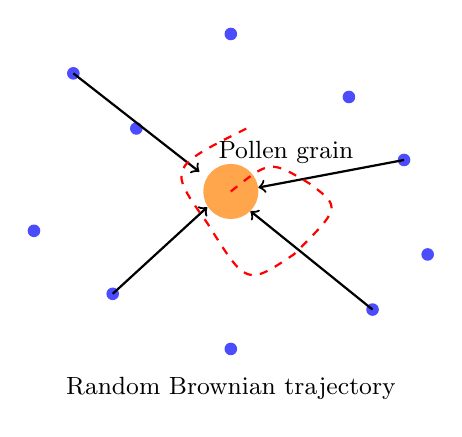
\begin{tikzpicture}
            % water molecules
            \foreach \x/\y in {
            -2/1.5,
            -1.2/0.8,
            -2.5/-0.5,
            -1.5/-1.3,
            1.5/1.2,
            2.2/0.4,
            2.5/-0.8,
            1.8/-1.5,
            0/2,
            0/-2
            }
            {
                \fill[blue!70] (\x,\y) circle (0.08);
            }

            % pollen grain
            \fill[orange!70] (0,0) circle (0.35);

            % random impacts
            \draw[->,thick] (-2,1.5) -- (-0.4,0.25);
            \draw[->,thick] (-1.5,-1.3) -- (-0.3,-0.2);
            \draw[->,thick] (2.2,0.4) -- (0.35,0.05);
            \draw[->,thick] (1.8,-1.5) -- (0.25,-0.25);

            % trajectory
            \draw[dashed,red,thick]
            (0,0)
            .. controls (0.5,0.4) .. (1,0.1)
            .. controls (1.4,-0.2) .. (0.8,-0.8)
            .. controls (0.2,-1.2) .. (-0.3,-0.4)
            .. controls (-0.8,0.3) .. (0.2,0.8);

            \node at (0,-2.5) {\small Random Brownian trajectory};
            \node at (0.7,0.5) {\small Pollen grain};
        \end{tikzpicture}

        Illustration of Brownian motion. A microscopic pollen grain suspended in a fluid is continuously struck by surrounding molecules. Because the collisions occur randomly and from different directions, the grain follows an irregular trajectory (red dashed line). Brownian motion provides direct evidence that matter at finite temperature is constantly moving at the microscopic scale.
    \end{center}

    \highspace
    \textcolor{Green3}{\faIcon{question-circle} \textbf{How is linked to thermal energy?}} Brownian motion is a direct consequence of the thermal energy of the surrounding environment. At finite temperature, particles in a fluid are in constant motion due to their thermal energy. This motion leads to random collisions with suspended particles, causing the observed Brownian motion. The intensity of Brownian motion increases with temperature, as higher thermal energy results in more vigorous particle movement and more frequent collisions. Indeed, if we boil the water, the Brownian motion becomes more pronounced as the water molecules move faster and collide more frequently with the pollen grain.

    \highspace
    \textcolor{Green3}{\faIcon{question-circle} \textbf{Amazing, but how is it relevant for quantum computing?}} The actual \textbf{enemy is not Brownian motion} itself, but the fact that the \textbf{thermal environment constantly interacting with the qubit}. Brownian motion is simply an intuitive \hl{example showing that matter at finite temperature is never perfectly still, but rather in constant motion}. This means that \textbf{qubits are continuously affected by their environment}, leading to errors in quantum computations. Even if we try to isolate the qubits as much as possible, they will still be subject to random disturbances from the surrounding environment, making it impossible to achieve perfect error-free quantum computation.
\end{examplebox}

\begin{flushleft}
    \textcolor{Green3}{\faIcon{question-circle} \textbf{Why Error Correction is necessary}}
\end{flushleft}
Quantum algorithms often require millions of gate operations. Without a protection mechanism, continuous interaction with the environment would cause decoherence (\autopageref{sec:decoherence}) and accumulate gate errors (\autopageref{sec:gate-infidelity}) during computation, making it \textbf{highly unlikely that the correct result would be obtained}.

\highspace
However, there is hope. The \textbf{Threshold Theorem} (\autopageref{def:threshold-theorem}) discussed previously provides the curcial insight that reliable \textbf{quantum computation is still possible} if errors are corrected continuously and the physical error rate remains below a certain threshold.

\highspace
For this reason, modern quantum computers cannot rely solely on physical qubits (\autopageref{sec:logical-vs-physical-qubits}). Instead, they require \textbf{Quantum Error Correction Codes} (QECCs), which encode quantum information redudantly across many physical qubits in order to detect and correct errors before they destroy the computation.
\begin{align*}
    \text{\textcolor{Red2}{\faIcon{exclamation-triangle}}} \hspace{1em} & \text{Noise} \to \text{Errors} \to \text{Decoherence} \to \text{Computation Failure} \\
    \text{\textcolor{Green3}{\faIcon{check-circle}}}       \hspace{1em} & \text{Noise} \to \text{Quantum Error Correction} \to \text{Reliable Computation}
\end{align*}